\documentclass[a4paper,10pt, bibliography=totocnumbered]{scrreprt}

\usepackage[utf8x]{inputenc}
\usepackage[english]{babel}

\usepackage{graphicx}
\usepackage{pdfpages}
%\usepackage{subfig}
%\usepackage{microtype}
\usepackage{tabularx}
%\usepackage{amsmath, textcomp}

% Custom packages
\usepackage[numbers]{natbib}
\usepackage{longtable}
\usepackage{ragged2e}
%\usepackage{tikz}
%\usetikzlibrary{positioning}
%\usepackage{pdflscape}
%\usepackage{rotating}

\usepackage{glossaries} 

\usepackage{hyperref}
\hypersetup{
    colorlinks=true,        % false: boxed links; true: colored links
    linkcolor=black,        % color of internal links
%    citecolor=green,        % color of links to bibliography
    citecolor=black,        % color of links to bibliography
    filecolor=magenta,      % color of file links
    urlcolor=blue           % color of external links
}


%% Title Page
\makeatletter
\renewcommand{\maketitle}{\begin{titlepage}
    \vskip 10\p@
    \hbox{
      \vrule depth 0.99\textheight
        \mbox{\hspace{2em}}
      \vtop{
        \vskip 10\p@
        \hspace{4pt}
        \vskip 50\p@
        \begin{flushleft}
          \Large \@author \par
        \end{flushleft}
        \vskip 50\p@
        \begin{flushleft}
          \huge \bfseries \@title \par
        \end{flushleft}
        \begin{flushleft}
          \Large \bfseries \@subtitle \par
        \end{flushleft}
        \vskip 70\p@
        \begin{flushleft}
          \Large \@publishers \par
        \end{flushleft}
        \vskip 50\p@
        \begin{flushleft}
          \Large \@date \par
        \end{flushleft}
        }}
  \end{titlepage}
}
\makeatother

\author{Lucienne-Sophie Marmé}
\title{Requirements identification in Twitter data}
\publishers{\textbf{Advisor University of Heidelberg}\\ Prof. Dr. Barbara Paech, Michael Anders}
\date{\today}



% Deutsche Absaetze:
\parindent 0pt
\parskip 12pt

\textwidth145mm
\setlength{\oddsidemargin}{0.7cm}
\setlength{\topmargin}{-0.5cm}
\setlength{\textheight}{22.5cm}

\begin{document}
\maketitle


\begin{abstract}
\section*{Abstract}
Building on results of previous research which show that users employ Twitter – one of the most popular social networks – to communicate about software application via so called tweets (short messages), in this paper we discuss two approaches that aim to use technical related tweets to extract relevant information from end-users for maintaining software quality and requirements engineering. Motivated by the large number of tweets published on a daily base – in the range of 30,000 for popular applications such as Facebook and Snapchat, and the large number of tweets not containing any requirements-related information, the two chosen approaches are looking for an automatic way to extract, process, analyze and summarize software-related tweets.
\end{abstract}


\tableofcontents

\chapter{Introduction}

Connecting with customers or users to get feedback for released products always has been one of the most effective ways to build and develop a product the user actually likes and uses. Collecting feedback is crucial concerning not only to maintain the quality of the product but to increase the functionalities and usability. There are many established feedback streams like App Store reviews or blogs where users can directly report issues and request new features. 
With the rise of social media a completely new tool for developers to connect with their end users comes to light. One might ask why leveraging the last possible way of extracting user feedback. The answer is simple, with over 2.25 million active apps alone within the Apple App Store (March 2015) and a growth of 1000 apps per day, the way of staying in competition as a software owner and developer is to connect constantly with the users of the product (G. Williams et al. \cite{Williams}). That being said Twitter as one of the most popular social networks has lots of potential and offers a great opportunity to extend traditional feedback sources. The results of the work of E. Guzman et al. \cite{Guzman} show that with the same amount of tweets and app store reviews (1,350) 42\% of the tweets directed to support accounts had technical relevant information for software evolution in comparison to the app store where only 34\% of the reviews contained technical useful information. Twitter due to it's nature as a broadly used communication tool has the advantage of being able to address a large audience and lowering the inhibitions of people to feedback certain things because as Twitter is no limited to feedback they often don't need to change their context to do so. Additionally the end users are able to connect directly with the developers and vice versa.
In this chapter we are looking at two approaches that are aiming at leveraging Twitter as a new feedback source to collect technical useful information for software evolution.

All technical terms used in this report can be found in the glossary with more detailed explanations.


\chapter{Literature Search}
\label{chap:2}

The center of the literature search is the research question which for this case reads as follows:
\textit{What approaches for identifying requirements in Twitter data are there and what type of requirements can be identified?}

Out of the research question singular search expressions can be extracted like \textit{Requirement(s), "Requirement(s) Identification /Classification /Extraction", "Software Evolution", "Twitter Data", "Mining Tweets", Twitter, "Twitter Feeds"} in order to form search requests. 

As for the search tools, IEEE, ATM and Elsevier are used.
To start the search some basic criteria are set to determine the relevance and quality of a paper:

\begin{enumerate}
    \item The paper should preferably be written in English because English is the common language in computer science.
    \item The paper should be fairly new (not older than five years) in order to still be relevant.
    \item The paper describes an approach to identify, classify and extract software-relevant tweets
\end{enumerate}

The above mentioned search expression are the basis of the search. Using the advanced filter tool of the chosen search tools all of the criteria and different combinations of the search expressions can be entered and analysed. The results are shown in the table below (Figure 2.1: \textit{Literature Search Plan})

Systematically this procedure contains the following steps: 
Firstly note all possible combination possibilities in one column and add additional columns for each used search tool. Then for each search request note the number of hits obtained with each of the search tools. If the number of hits is to high to look through each of the papers name limit the search request, e.g set the publication date to the last year so only paper published within the last year are shown. The other way around if no results were found extent for example the keyword search to not only the title but also the abstract.
If the number of papers is now manageable (around 50 papers) go through the list of titles and write down titles that capture the elements of the research question. If the title isn't enough look at the abstract as well to get a sense of what the paper is covering. Every time a paper seems to match the criteria make a note in the table. After going through all different search requests take a look at all noted papers. And write down why a paper is suitable for answering the research question or why not. 

As a result of this search the work of Guzman et al.\cite{Guzman} and Williams et al.\cite{Williams} is chosen because they fill all criteria especially the last one namely giving an approach or analysis on how to identify, classify and extract software-relevant information from twitter. 

\begin{figure}
\centering
\includegraphics[scale=0.4]{images/Thema_5_LiteratureSearch.png}
\caption{Literature Search Plan}
\label{fig:literatureSearchPlan}
\end{figure}



\chapter{A Little Bird Told Me: Mining Tweets for Requirements and Software Evolution}
\label{chap:3}

\section{Goal}

Since Twitter is one of the most popular social networks this paper concentrates on an approach to automatically classify, group and rank tweets about software applications. The so-called ALERTme approach describes a way of exploiting Twitter as a feedback channel for retrieving software evolution relevant information especially including end-user requirements. To do so three main steps are performed:
\begin{enumerate}
    \item Classifying tweets into categories related to software evolution
    \item Grouping tweets according to their content
    \item Ranking tweets according to their relevance
\end{enumerate}

\section{Algorithm}
As a basis for the main steps of the ALERTme approach by E. Guzman et al. \cite{Guzman} the data is preprocessed by tokenizing the tweets, converting all text into lower case, extracting n-grams with one to three word length, removing stopwords and finally stemming the text, thus eliminating inflectional forms of words. 

In order to classify the tweets into two chosen categories: \textit{improvement request} and \textit{other} supervised machine learning techniques were used to do so automatically. In particular Multinomial Naive Bayes (MNB) is used for the classification task. To train the classifiers the preprocessed tweet text is converted into a vector space model using TF-IDF as a weighting scheme. After that the classifiers are trained on a set of manually labeled tweets.

For grouping the ALERTme approach by E. Guzman et al. \cite{Guzman} uses the Biterm Topic Model (BTM), a topic modeling algorithm. This algorithm takes as input the preprocessed text of each tweet and outputs the topics (groups of words) that co-occur in the whole corpus of tweets and the association between the tweets and topics in form of a probability matrix.

In order to rank the tweets and determine the individual relevance of each tweet and topic a weighted function is used. Thereby considering elements like category, retweets, likes, sentiment, social rank and duplicates to calculate the individual ranking.

 \[ TWR(tw) = \sum_{i=1}^{6} w_i * f_i(tw) \] 

\begin{figure}
\centering
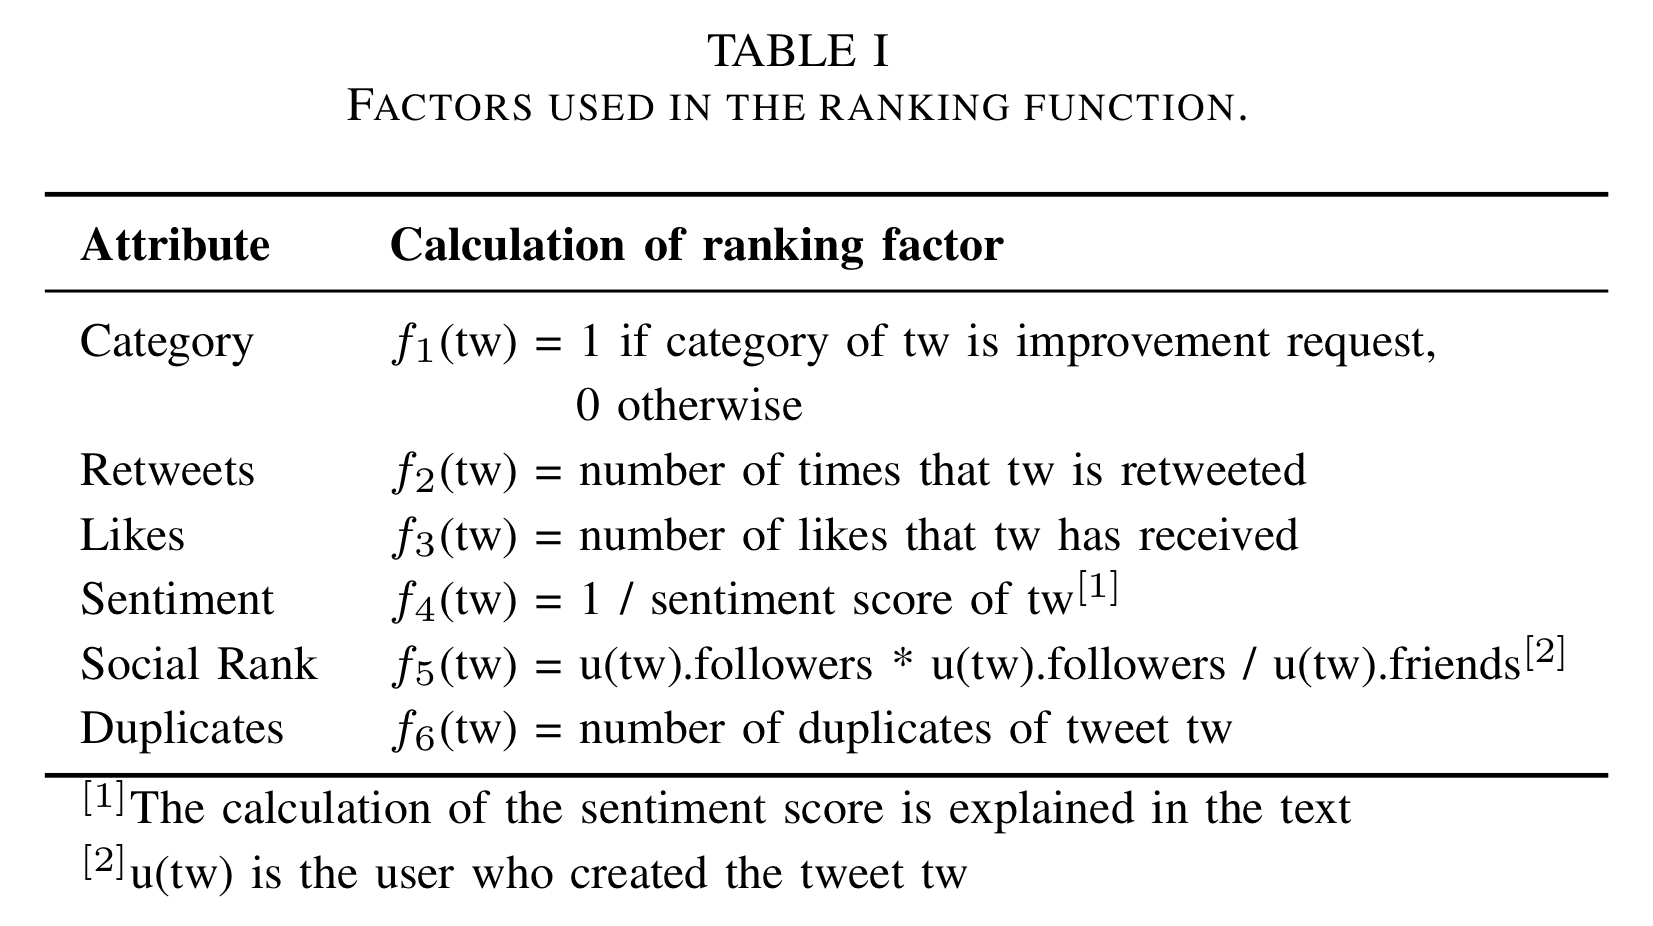
\includegraphics[scale=0.2]{images/Thema_5_RankingFunction.jpeg}
\caption{Overview of factors used in the ranking function}
\label{fig:RankingFunction}
\end{figure}

There are six different factors that contribute to the individual ranking score (see the table above, Figure 3.1: \textit{Overview of factors used in the ranking function}). To calculate the sentiment score of tweets SentiStrength is used. This lexical sentiment analysis tool assigns both a positive and a negative score with ranges of [1, 5] and [-1, -5] to each tweet. 5 denotes an extremely positive and -5 and extremely negative sentiment. To calculate the final score both of these scores are added up and then 5 is added as well. As tweets with low sentiment score typically require more attention, the inverse of the sentiment score is used.

\section{Evaluation}

The evaluation of the ALERTme approach is divided into three main parts: Classification, grouping and ranking. To determine the accuracy of each step a dataset containing 68,108 tweets from support accounts of  Slack, Spotify and Dropbox is created. 

To evaluate the first part namely the classification a manually created truthset consisting out of 1,350 tweets is used to compare two different classifiers: The before mentioned Multinomial Naive Bayes classifier and the Random Forest classifier. To evaluate the performance of both classifiers traditionally used metrics like precision, recall and F-measure are used.
The results in figure 3.2: \textit{Classification results} show that though both classifier deliver encouraging results, the Random Forest classifier is outperformed by the Multinomial Naive Bayes classifier on the F-measure.

\begin{figure}
\centering
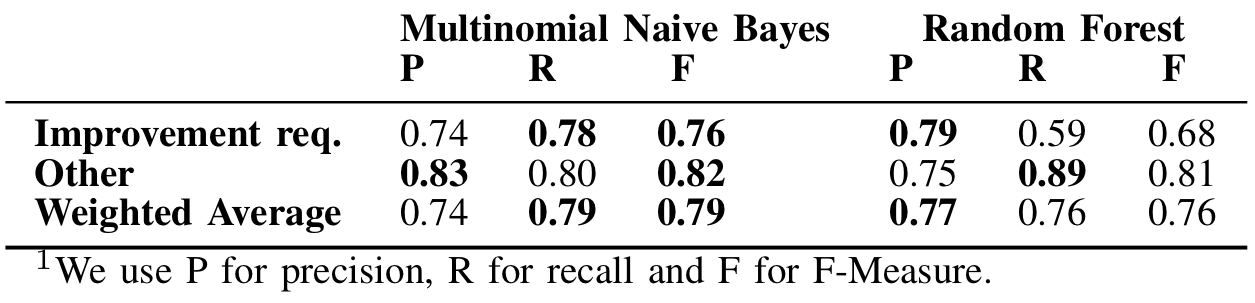
\includegraphics[scale=0.2]{images/Thema_5_approach_1_classification.jpeg}
\caption{Classification results}
\label{fig:RankingFunction}
\end{figure}

Concerning the grouping aspect of the ALERTme approach by E.Guzman et al. \cite{Guzman} two experiments are conducted: The word intrusion task which evaluates the semantic coherence of the topics (given by the topic modeling algorithm) and the topic intrusion task which tests the accuracy of the association between topics and tweets according to human judgement.
The results of the BTM algorithm were compared to the results of the Latent Dirichlet Allocation (LDA) algorithm. As metrics Model Precision (MP) and Topic Precision (TP) were used. Where MP defines the proportion of participants concurring with the topic model with respect to which word is considered an intruder. Analog, TP defines the same but with respect to which topic is considered an intruder.
The results show that the association accuracy between topics and tweets is strong and the coherence of the generated topics is reasonable. Overall, BTM outperforms LDA.

The focus of evaluating the ranking step of the ALERTme by E.Guzman et al. \cite{Guzman} approach lays on the assessment of the used weights within the weighted function. To do so, a manually created truthset is used and compared to the results of the automatically created ranking scores using different weighting schemes. Overall, the results of the ranking step with the different weighting schemes are encouraging.


\chapter{Mining Twitter Feeds for Software User Requirements}
\label{chap:4}

\section{Goal}
The goal of this paper is similar to the motivation of the first approach by E. Guzman et al. \cite{Guzman}. In particular the main focus is on the evaluation of the performance of multiple data classification and summarization techniques in automatically detecting and summarizing technical user concerns raised in software-relevant tweets. The main goal hereby is to support an adaptive date-driven requirements engineering process that can detect user's needs in an effective and timely manner. In order to examine the value of Twitter as a source of feedback that can be helpful for software evolution the following three research questions are discussed in this paper: 

\begin{enumerate}
    \item RQ1: \textit{How informative is Twitter data for software engineers?}
    \item RQ2: \textit{To what extent can informative software-relevant tweets be automatically classified?}
    \item RQ3: \textit{How can informative tweets be accurately summarized?}
\end{enumerate}

\section{Algorithm}
To determine the information value of the data, the sampled data is manually analysed by industry professionals. The categories in which the tweets were categorized were \textit{bug reports, user requirements and miscellaneous and spam}. Overall, the manual analysis shows that out of 4000 tweets, 51\% were technically informative (27\% big reports, 24\% user requirements) while the other 49\% were categorized as spam and miscellaneous. 

In order to see which classifier proves to be the most effective and which classification features generate the most accurate results two classification algorithms were analyzed. Firstly the Naive Bayes (NB) classifier and secondly the Support Vector Machines (SVM) classifier. Regarding the classification features textual content (BOW), text processing techniques including stemming, stopword removal and sentiment analysis were used.

Concerning the realisation of summarizing technically informative tweets the work of Grant Williams and Anas Mahmoud \cite{Williams} examines three different extractive summarization techniques: Hybrid Term Frequency (TF), Hybrid TF.IDF and SumBasic.


\section{Evaluation}

The qualitative analysis of the data revealed that about 50\% of the tweets contained useful technical data.
To evaluate the two chosen classifiers the same metrics as in the approach of Guzman et al. \cite{Guzman} are used: Recall (R), precision (P) and F-measure (F).

In terms of classifier' accuracy as seen in Figure 4.1: \textit{Summary of classification accuracy} both SVM and NB were able to achieve competitive results and showed that NB as well as SVM can be effective in capturing and categorizing software-related tweets. Regarding the classification features, sentiment analysis showed no impact on performance whereas text reduction strategies like stemming and stopword removal had conflicting impact on the classification accuracy.
This can be attributed to the fact that software-related tweets tend to be neutral. While bugs tend to be slightly more negative and requirements slightly more positive the difference is not enough to affect the classification accuracy as shown in Figure 4.2: \textit{Sentiment scores for bug reports, user requirements, and other tweets}.

To assess the quality of the different summarization algorithms an experiment with ten programmers (including 3 graduate students in computer science and 7 industry professionals) is conducted. 
Therefore, five systems were randomly selected. For each system two sets of tweets, including the set of bug reporting and the set of user requirement tweets were provided. The main task for the experts consists of going through each set and identify 10 tweets that they believe capture the common concerns raised in the set. 
To assess the quality of the automatically created summaries, for each system, the average term overlap between the experts' selected lists of tweets (reference summaries) and the various automatically generated summaries are calculated. Meaning that an automated summary that contains a greater number of terms from the reference summary is considered more effective. 
SumBasic proves to be the most successful of the three evaluated algorithms.

\begin{figure}
\centering
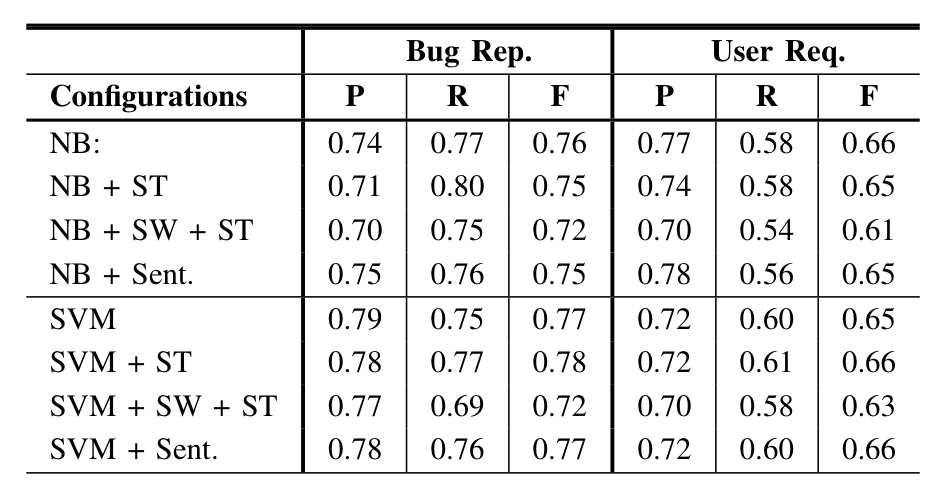
\includegraphics[scale=0.2]{images/Thema_5_approach_2_accuracy.jpeg}
\caption{Summary of classification accuracy}
\label{fig:Summary of classification accuracy}
\end{figure}

\begin{figure}
\centering
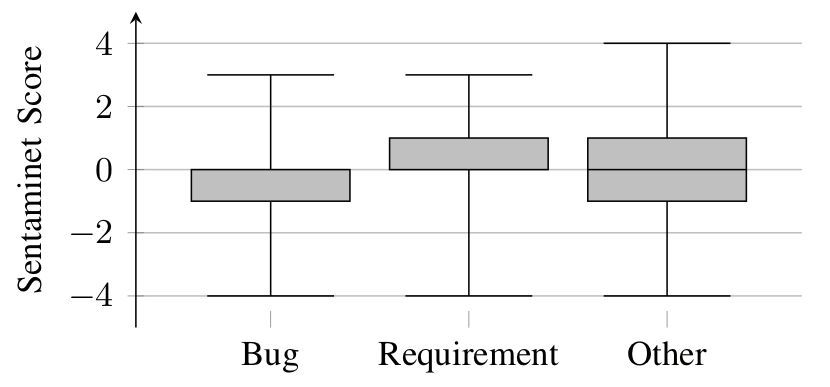
\includegraphics[scale=0.2]{images/Thema_5_approach_2_sentiment.jpeg}
\caption{Sentiment scores for bug reports, user requirements, and other tweets}
\label{fig:Summary of classification accuracy}
\end{figure}


\chapter{Comparison}

\section{Synthesis}
The ALERTme approach by E. Guzman et al. \cite{Guzman} is focused on filtering, summarizing and ranking tweets about software applications. As a result, allowing stakeholders to use Twitter as a feedback channel for software evolution, including end-user requirements. The approach presented in the paper “Mining Twitter Feeds For Software User Requirements” by G. Williams et al. \cite{Guzman} also aims at leveraging Twitter as a main source of useful software user feedback but focuses on evaluating the performance of multiple data classification and summarization techniques in automatically detecting and summarizing technical user concerns.


The ALERTme approach by E. Guzman et al. \cite{Guzman} is relying on the following methods for preprocessing, classifying, grouping, and ranking their data: tokenizing, removing stop words, stemming, Supervised Machine Learning, Multinomial Naïve Bayes (MNB), TF-IDF, Biterm Topic Model (BTM), weighted function (TWR), SentiStrength. 

In course of answering the research questions of the work of G. Williams et al. \cite{Williams} variety of methods are used, like Naïve Bayes (NB), Support Vector Machines (SVM), bag-of-words (BOW), stemming (ST), stop-word (SW) removal, Sentiment Analysis, hybrid TF, hybrid TF.IDF, SumBasic.

The main goals of the ALERTme approach by E. Guzman et al. \cite{Guzman} are to filter tweets that do not contain information relevant for their tasks, further summarize tweet content, thus simplifying the task of identifying requirements or other information relevant for software evolution and obtain information about the relevance of the tweets which, for example, can be used for prioritizing requirements elicited from the tweets. 

Whereas the approach by G. Williams et al. \cite{Williams} is focused on determining how technically informative, or useful, software user’s tweets are and detecting the degree of automatization concerning classifying informative software-relevant tweets. Additionally possible ways of summarization informative tweets are discussed.


Both the ALERTme approach by E. Guzman et al. \cite{Guzman} and the approach by G. Williams et al. \cite{Williams} are focused on short, informal feedback with social components available on Twitter.


Concerning the parts of software development process which are supported by the ALERTme approach by E. Guzman et al. \cite{Guzman} the focus is on maintaining software quality and identifying ideas for improvement. The second approach by G. Williams et al. \cite{Williams} targets the development of actionable software engineering requests on basis of Twitter feedback. And helping software developers to connect with their users instantly and directly. The supported stakeholders of the ALERTme approach by E. Guzman et al. \cite{Guzman} are developers, requirements engineers and product owners. Whereas the other approach by G. Williams et al. \cite{Williams} mainly focuses on supporting developers.


The evaluation of the ALERTme approach by E. Guzman et al. \cite{Guzman} is divided into three subcategories: Classification, grouping and ranking. 


As for evaluating the classification process of the ALERTme approach a truthset is manually created containing 1,350 tweets. 
On basis of the truthset the classifiers were trained and tested with 10-fold cross validation. The result achieved with the Multinomial Naïve Bayes were compared against the results of the Random Forest classifier.


Regarding the evaluation of the grouping aspect the topic intrusion task is used to determine if the association between topics and tweets are accurate according to human judgement. The results were compared against the results produced by the Latent Dirichlet Allocation (LDA) algorithm and the BTM algorithm.


To evaluate the ranking part of the ALERTme approach by E. Guzman et al. \cite{Guzman} the results from the ranking step are compared against the judgement of software practitioners. 

As a result, the ALERTme approach by E. Guzman et al. \cite{Guzman} can automatically classify tweets into two categories (improvement request and other categories) with a F-Measure of 0.79, group tweets into groups which have a reasonable coherence and the association quality between the generated topics and analyzed tweets is very satisfactory and lastly rank tweets where the ranking results strongly agree with practitioner’s judgement.


The evaluation of the the work by G. Williams et al. \cite{Williams} is also divided but in this case into two parts: Classification and summarization.

The classifiers were trained with 10-fold cross validation. The same metrics as in the evaluation of the ALERTme approach by E. Guzman et al. \cite{Guzman} are used within this evaluation to evaluate the performance: Recall, precision F-measure.

To assess the quality of the different summarization algorithms an experiment as mentioned before in 3.2 is conducted.

The results of the evaluation show around 50\% of the sampled tweets contained useful technical data that can be translated into actionable bug reports and user requirements. In addition, NB and SVM are proven to be effective in capturing and categorizing software-related tweets. Concerning the classification features Sentiment Analyses seems to have no impact on performance, while text reduction strategies have a conflicting impact on the classification accuracy. As for the summarization algorithm evaluation “SumBasic” was the most successful algorithm.

\pagebreak
\section{Synthesis matrix}
\begin{center}
\begin{tabular}{ | m{4em} | m{1,9cm}| m{5cm} | m{5cm} | } 
  \hline
  Synthesis question no. & Synthesis question & ALERTme & Grant Williams, Anas Mahmoud \\ 
  \hline
  3-a & Used methods & \begin{enumerate}
    \item Preprocessing: Tokenizing, extracting n-grams, stop word removal and stemming the text
    \item Classification: Multinomial Naive Bayes (MNB), TF-IDF 
    \item Grouping: Biterm Topic Model (BTM)
    \item Ranking: SentiStrenght
\end{enumerate} & \begin{enumerate}
    \item Classification:Naive Bayes (NB), Support Vector Machines (SVM)
    \item Classification Features:Bag-of-words, Stemming, Stop word removal, Sentiment Analysis
    \item Summarization: hybrid TF, hybrid TF.IDF, SumBasic
\end{enumerate} \\ 
  \hline
  3-b & Classification goal of the approach & create an approach to filter, group and rank tweets & (Qualitative) analysis of Twitter data, degree of automatization concerning classification and ways of summarization \\ 
  \hline
  3-c & Requirements and constraints for data and approach	 & short, informal text with social components (Twitter)
 & short, informal text with social components (Twitter)
 \\ 
  \hline
  4-a & Supported development procedures & Development, Quality Management, Requirements Engineering
 & Requirements engineering process (Development) \\ 
  \hline
  4-b & supported stakeholders & Developers, requirements engineers or product owners & Developers \\ 
  \hline
  5-a & Tool support/prototypes & none & none \\ 
  \hline
  5-b & Degree of automation & Fully automatable & The results of the analysis show that the process could be fully automatable \\ 
  \hline
\end{tabular}
\end{center}

\begin{center}
\begin{tabular}{ | m{4em} | m{1,9cm}| m{5cm} | m{5cm} | } 
  \hline
  Synthesis question no. & Synthesis question & ALERTme & Grant Williams, Anas Mahmoud \\ 
  \hline
    6-a & Evaluation of the approach & \begin{enumerate}
    \item Classification: Comparison of automatic classification against a manually generated truthset (1,350 Tweets)
    \item Grouping: executed two assessment tasks for systematically determining the quality of the tweet groups according to software practioners` judgement 
    \item Ranking: Evaluated ranking function against the assessment of software practitioners 
\end{enumerate} & \begin{enumerate}
    \item Classification: Comparison of automatic classification against a manually generated truthset (4,000 Tweets)
    \item Summarization: Evaluated summarization algorithms the assessment of software practitioners
\end{enumerate} \\ 
  \hline
    6-b & Key evaluation results & \begin{enumerate}
    \item Classification: MNB outperforms Random Forest with: F-Measure of 0.79 
    \item Grouping: Association quality between the generated topics and analyzed tweets is very satisfactory

    \item Ranking: Ranking step produces results that strongly agree with practitioners' judgement 
\end{enumerate} & \begin{enumerate}
    \item Qualitative: Around 50\% contained useful technical data
    \item Classification: Analysis showed that NB and SVM can be effective in capturing and categorizing software-related tweets
    Classification features: 
    Sentiment Analyses -> no impact on performance
    Text reduction strategies -> conflicting impact on the classification accuracy

    \item Summarization: “SumBasic” most successful summarization algorithm
\end{enumerate} \\ 
  \hline
\end{tabular}
\end{center}
\label{chap:5}

\section{Comparison}
Both approaches aim at the exploitation of Twitter as a feedback channel for software relevant information including end-user requirements. Therefore, both approaches use a lot of the same methods for example regarding the text processing (stemming and stop word removal) and the classification process where both use supervised machine learning techniques. In terms of grouping/summarizing the extracted data both approaches use different techniques to come to their results. The ALERTme approach by E. Guzman et al. \cite{Guzman} uses a topic modeling algorithm (BTM) specialized in short text for grouping semantically related tweets and then ranking them with a weighted function. Whereas the second approach by G. Williams et al. \cite{Williams} is using different summarization algorithms like “SumBasic” to summarize technical user concerns. Both approaches focus on short, informal text with social components available on Twitter and aim to support the same steps of software development. The work of G. Williams et al. \cite{Williams} solely focuses on supporting developers whereas the ALERTme approach also explicitly name requirement engineers and product owners. Both are fully automated and use for evaluating their classification processes the same metrics but compare different classifiers with another. As mentioned before the grouping and ranking part of the ALERTme approach by E. Guzman et al. \cite{Guzman} differs from the summarization part of the approach by G. Williams et al. \cite{Williams}. 

In conclusion, both approaches present different methods for requirements identification on basis of Twitter data. As both papers focus on different aspects of the process it depends on which suits your application the best.

\chapter{Conclusion}
\label{chap:6}

Even though both approaches showed that looking at Twitter as a new source of feedback opens up a lot of new capacities it also came across with the many difficulties that come along due to nature of Twitter and tweets. Such as, dealing with short and informal text, process millions of messages per day etc.
The work of E. Guzman et al. \cite{Guzman} focuses on building a approach to manifest a specific procedure to extract, classify and rank tweets. Whereas the work of G. Williams et al. \cite{Williams} concentrates on answering research questions regarding Twitter as a new feedback channel and evaluate different methods to classify and summarize technical relevant tweets. There are many commonalities for example using some of the same techniques for classifying tweets etc. 
But there are also differences, E. Guzman et al. \cite{Guzman} include a ranking procedure in their work whereas the work of G. Williams et al. \cite{Williams} does not but therefore evaluates methods for summarizing tweets.
Overall, the results of both approaches are promising and form a solid base for future work.


%% Bibliography
\bibliographystyle{plainnat}
%\bibliography{literature.bib}%Bibliography file name

\begin{thebibliography}{9}

\bibitem{Guzman} Emitza Guzman, Mohamed Ibrahim and Martin Glinz. 2017. A Little Bird Told Me: Mining Tweets for Requirements and Software Evolution. In Proceedings of the 25st IEEE International Requirements Engineering Conference.
DOI: 10.1109/RE.2017.88. INSPEC Accession Number: 17207678. Date of Conference: 4-8 Sept. 2017. Conference Location: Lisbon, Portugal.


\bibitem{Williams} Grant Williams and Anas Mahmoud, Mining Twitter Feeds for Software User Requirements. 2017 International Requirements Engineering Conference.
DOI: 10.1109/RE.2017.14. INSPEC Accession Number: 17207626. Date of Conference: 4-8 Sept. 2017. Conference Location: Lisbon, Portugal.
\end{thebibliography}

\listoffigures

%\listoftables

\end{document}          
